% A standalone TikZ figure. Compiling produces just the image (cropped to the
% drawing), so the preview is the figure itself. Draw with the visual editor or
% edit the TikZ here, then reuse the compiled figure in any document.
\documentclass[tikz,border=6pt]{standalone}
\usepackage{tikz}
\usetikzlibrary{shapes.geometric,arrows.meta,positioning,calc,backgrounds}

\begin{document}
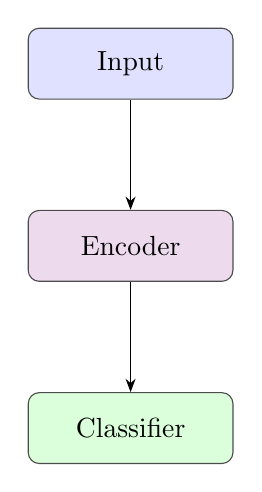
\begin{tikzpicture}[>=Stealth, node distance=1.4cm,
    box/.style={draw=black!70, rounded corners, minimum width=2.6cm,
                minimum height=0.9cm, align=center}]
  \node[box, fill=blue!12] (input) {Input};
  \node[box, fill=violet!14, below=of input] (encoder) {Encoder};
  \node[box, fill=green!14, below=of encoder] (classifier) {Classifier};
  \draw[->] (input) -- (encoder);
  \draw[->] (encoder) -- (classifier);
\end{tikzpicture}
\end{document}
